\documentclass{standalone}
\usepackage{tikz}
\usetikzlibrary{patterns, positioning}
\usetikzlibrary{shapes.misc}
\usepackage[outline]{contour}
\contourlength{1.5pt} 


\begin{document}
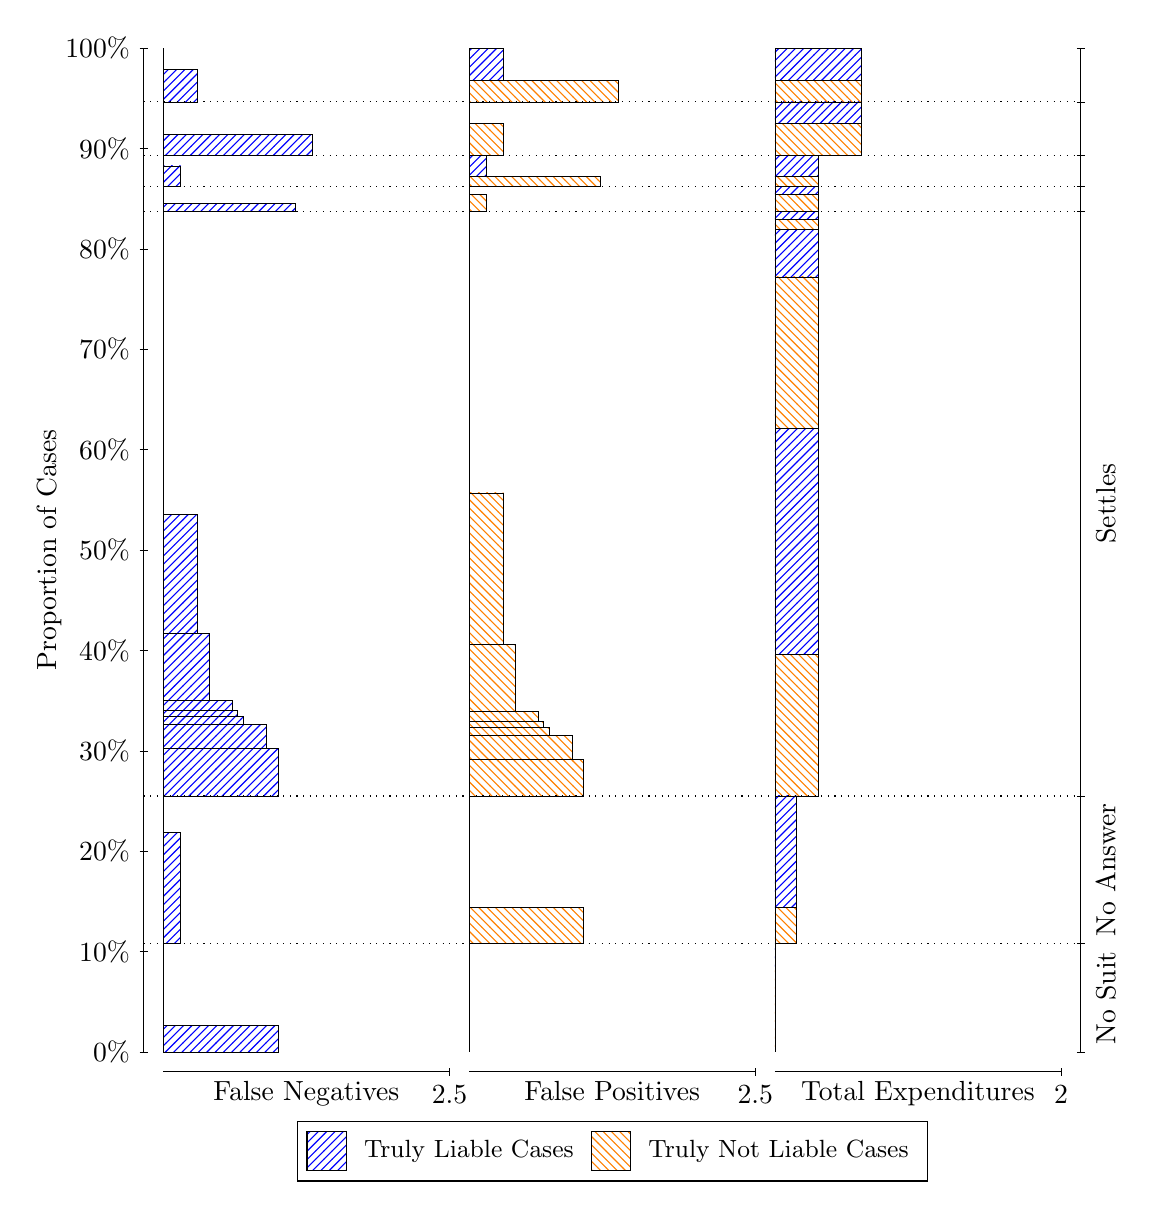
\begin{tikzpicture}
\draw[black, very thin] (1.5,1.75) -- (1.5,14.5);
\node[rotate=90, text=black, anchor=center] at (0.3, 8.125) {Proportion of Cases};
\draw[black, very thin] (1.45,1.75) -- (1.55,1.75);
\node[text=black, anchor=east] at (1.45, 1.75) {0\%};
\draw[black, very thin] (1.45,3.025) -- (1.55,3.025);
\node[text=black, anchor=east] at (1.45, 3.025) {10\%};
\draw[black, very thin] (1.45,4.3) -- (1.55,4.3);
\node[text=black, anchor=east] at (1.45, 4.3) {20\%};
\draw[black, very thin] (1.45,5.575) -- (1.55,5.575);
\node[text=black, anchor=east] at (1.45, 5.575) {30\%};
\draw[black, very thin] (1.45,6.85) -- (1.55,6.85);
\node[text=black, anchor=east] at (1.45, 6.85) {40\%};
\draw[black, very thin] (1.45,8.125) -- (1.55,8.125);
\node[text=black, anchor=east] at (1.45, 8.125) {50\%};
\draw[black, very thin] (1.45,9.4) -- (1.55,9.4);
\node[text=black, anchor=east] at (1.45, 9.4) {60\%};
\draw[black, very thin] (1.45,10.675) -- (1.55,10.675);
\node[text=black, anchor=east] at (1.45, 10.675) {70\%};
\draw[black, very thin] (1.45,11.95) -- (1.55,11.95);
\node[text=black, anchor=east] at (1.45, 11.95) {80\%};
\draw[black, very thin] (1.45,13.225) -- (1.55,13.225);
\node[text=black, anchor=east] at (1.45, 13.225) {90\%};
\draw[black, very thin] (1.45,14.5) -- (1.55,14.5);
\node[text=black, anchor=east] at (1.45, 14.5) {100\%};

\draw[black, very thin] (13.4,1.75) -- (13.4,14.5);
\draw[black, very thin] (13.35,1.75) -- (13.45,1.75);
\node[anchor=west] at (13.35, 1.75) {};
\draw[black, very thin] (13.35,3.1254) -- (13.45,3.1254);
\node[anchor=west] at (13.35, 3.1254) {};
\draw[black, very thin] (13.35,5.001) -- (13.45,5.001);
\node[anchor=west] at (13.35, 5.001) {};
\draw[black, very thin] (13.35,12.428) -- (13.45,12.428);
\node[anchor=west] at (13.35, 12.428) {};
\draw[black, very thin] (13.35,12.742) -- (13.45,12.742);
\node[anchor=west] at (13.35, 12.742) {};
\draw[black, very thin] (13.35,13.134) -- (13.45,13.134);
\node[anchor=west] at (13.35, 13.134) {};
\draw[black, very thin] (13.35,13.817) -- (13.45,13.817);
\node[anchor=west] at (13.35, 13.817) {};
\draw[black, very thin] (13.35,14.5) -- (13.45,14.5);
\node[anchor=west] at (13.35, 14.5) {};

\draw[black, very thin, pattern color=blue, pattern=north east lines] (1.75,1.75) rectangle (3.2033,2.084);
\draw[black, very thin, pattern color=orange, pattern=north west lines] (1.75,2.084) rectangle (1.75,3.1254);
\draw[black, very thin, pattern color=blue, pattern=north east lines] (1.75,3.1254) rectangle (1.968,4.5411);
\draw[black, very thin, pattern color=orange, pattern=north west lines] (1.75,4.5411) rectangle (1.75,5.001);
\draw[black, very thin, pattern color=blue, pattern=north east lines] (1.75,5.001) rectangle (3.2033,5.6062);
\draw[black, very thin, pattern color=blue, pattern=north east lines] (1.75,5.6062) rectangle (3.058,5.909);
\draw[black, very thin, pattern color=blue, pattern=north east lines] (1.75,5.909) rectangle (2.7673,6.0119);
\draw[black, very thin, pattern color=blue, pattern=north east lines] (1.75,6.0119) rectangle (2.6947,6.0876);
\draw[black, very thin, pattern color=blue, pattern=north east lines] (1.75,6.0876) rectangle (2.622,6.2145);
\draw[black, very thin, pattern color=blue, pattern=north east lines] (1.75,6.2145) rectangle (2.3313,7.0636);
\draw[black, very thin, pattern color=blue, pattern=north east lines] (1.75,7.0636) rectangle (2.186,8.5783);
\draw[black, very thin, pattern color=orange, pattern=north west lines] (1.75,8.5783) rectangle (1.75,12.428);
\draw[black, very thin, pattern color=blue, pattern=north east lines] (1.75,12.428) rectangle (3.4213,12.53);
\draw[black, very thin, pattern color=orange, pattern=north west lines] (1.75,12.53) rectangle (1.75,12.742);
\draw[black, very thin, pattern color=blue, pattern=north east lines] (1.75,12.742) rectangle (1.968,13.004);
\draw[black, very thin, pattern color=orange, pattern=north west lines] (1.75,13.004) rectangle (1.75,13.134);
\draw[black, very thin, pattern color=blue, pattern=north east lines] (1.75,13.134) rectangle (3.6393,13.406);
\draw[black, very thin, pattern color=orange, pattern=north west lines] (1.75,13.406) rectangle (1.75,13.817);
\draw[black, very thin, pattern color=blue, pattern=north east lines] (1.75,13.817) rectangle (2.186,14.228);
\draw[black, very thin, pattern color=orange, pattern=north west lines] (1.75,14.228) rectangle (1.75,14.5);
\draw[black, very thin, pattern color=orange, pattern=north west lines] (5.6333,1.75) rectangle (5.6333,2.7914);
\draw[black, very thin, pattern color=blue, pattern=north east lines] (5.6333,2.7914) rectangle (5.6333,3.1254);
\draw[black, very thin, pattern color=orange, pattern=north west lines] (5.6333,3.1254) rectangle (7.0867,3.5854);
\draw[black, very thin, pattern color=blue, pattern=north east lines] (5.6333,3.5854) rectangle (5.6333,5.001);
\draw[black, very thin, pattern color=orange, pattern=north west lines] (5.6333,5.001) rectangle (7.0867,5.4699);
\draw[black, very thin, pattern color=orange, pattern=north west lines] (5.6333,5.4699) rectangle (6.9413,5.7727);
\draw[black, very thin, pattern color=orange, pattern=north west lines] (5.6333,5.7727) rectangle (6.6507,5.8756);
\draw[black, very thin, pattern color=orange, pattern=north west lines] (5.6333,5.8756) rectangle (6.578,5.9513);
\draw[black, very thin, pattern color=orange, pattern=north west lines] (5.6333,5.9513) rectangle (6.5053,6.0782);
\draw[black, very thin, pattern color=orange, pattern=north west lines] (5.6333,6.0782) rectangle (6.2147,6.9274);
\draw[black, very thin, pattern color=orange, pattern=north west lines] (5.6333,6.9274) rectangle (6.0693,8.8507);
\draw[black, very thin, pattern color=blue, pattern=north east lines] (5.6333,8.8507) rectangle (5.6333,12.428);
\draw[black, very thin, pattern color=orange, pattern=north west lines] (5.6333,12.428) rectangle (5.8513,12.639);
\draw[black, very thin, pattern color=blue, pattern=north east lines] (5.6333,12.639) rectangle (5.6333,12.742);
\draw[black, very thin, pattern color=orange, pattern=north west lines] (5.6333,12.742) rectangle (7.3047,12.872);
\draw[black, very thin, pattern color=blue, pattern=north east lines] (5.6333,12.872) rectangle (5.8513,13.134);
\draw[black, very thin, pattern color=orange, pattern=north west lines] (5.6333,13.134) rectangle (6.0693,13.545);
\draw[black, very thin, pattern color=blue, pattern=north east lines] (5.6333,13.545) rectangle (5.6333,13.817);
\draw[black, very thin, pattern color=orange, pattern=north west lines] (5.6333,13.817) rectangle (7.5227,14.089);
\draw[black, very thin, pattern color=blue, pattern=north east lines] (5.6333,14.089) rectangle (6.0693,14.5);
\draw[black, very thin, pattern color=orange, pattern=north west lines] (9.5167,1.75) rectangle (9.5167,2.7914);
\draw[black, very thin, pattern color=blue, pattern=north east lines] (9.5167,2.7914) rectangle (9.5167,3.1254);
\draw[black, very thin, pattern color=orange, pattern=north west lines] (9.5167,3.1254) rectangle (9.7892,3.5854);
\draw[black, very thin, pattern color=blue, pattern=north east lines] (9.5167,3.5854) rectangle (9.7892,5.001);
\draw[black, very thin, pattern color=orange, pattern=north west lines] (9.5167,5.001) rectangle (10.062,6.8005);
\draw[black, very thin, pattern color=blue, pattern=north east lines] (9.5167,6.8005) rectangle (10.062,9.6696);
\draw[black, very thin, pattern color=orange, pattern=north west lines] (9.5167,9.6696) rectangle (10.062,11.593);
\draw[black, very thin, pattern color=blue, pattern=north east lines] (9.5167,11.593) rectangle (10.062,12.198);
\draw[black, very thin, pattern color=orange, pattern=north west lines] (9.5167,12.198) rectangle (10.062,12.325);
\draw[black, very thin, pattern color=blue, pattern=north east lines] (9.5167,12.325) rectangle (10.062,12.428);
\draw[black, very thin, pattern color=orange, pattern=north west lines] (9.5167,12.428) rectangle (10.062,12.639);
\draw[black, very thin, pattern color=blue, pattern=north east lines] (9.5167,12.639) rectangle (10.062,12.742);
\draw[black, very thin, pattern color=orange, pattern=north west lines] (9.5167,12.742) rectangle (10.062,12.872);
\draw[black, very thin, pattern color=blue, pattern=north east lines] (9.5167,12.872) rectangle (10.062,13.134);
\draw[black, very thin, pattern color=orange, pattern=north west lines] (9.5167,13.134) rectangle (10.607,13.545);
\draw[black, very thin, pattern color=blue, pattern=north east lines] (9.5167,13.545) rectangle (10.607,13.817);
\draw[black, very thin, pattern color=orange, pattern=north west lines] (9.5167,13.817) rectangle (10.607,14.089);
\draw[black, very thin, pattern color=blue, pattern=north east lines] (9.5167,14.089) rectangle (10.607,14.5);
\draw[black, dotted] (1.5,3.1254) -- (13.4,3.1254);
\draw[black, dotted] (1.5,5.001) -- (13.4,5.001);
\draw[black, dotted] (1.5,12.428) -- (13.4,12.428);
\draw[black, dotted] (1.5,12.742) -- (13.4,12.742);
\draw[black, dotted] (1.5,13.134) -- (13.4,13.134);
\draw[black, dotted] (1.5,13.817) -- (13.4,13.817);
\draw[black, very thin] (1.75,1.5) -- (5.3833,1.5);
\node[text=black, anchor=north] at (3.5667, 1.5) {False Negatives};
\draw[black, very thin] (5.3833,1.45) -- (5.3833,1.55);
\node[text=black, anchor=north] at (5.3833, 1.45) {2.5};

\draw[black, very thin] (5.6333,1.5) -- (9.2667,1.5);
\node[text=black, anchor=north] at (7.45, 1.5) {False Positives};
\draw[black, very thin] (9.2667,1.45) -- (9.2667,1.55);
\node[text=black, anchor=north] at (9.2667, 1.45) {2.5};

\draw[black, very thin] (9.5167,1.5) -- (13.15,1.5);
\node[text=black, anchor=north] at (11.333, 1.5) {Total Expenditures};
\draw[black, very thin] (13.15,1.45) -- (13.15,1.55);
\node[text=black, anchor=north] at (13.15, 1.45) {2};

\node[text=black, centered, rotate=90] at (13.72, 2.4377) {\contour{white}{No Suit}};
\node[text=black, centered, rotate=90] at (13.72, 4.0632) {\contour{white}{No Answer}};
\node[text=black, centered, rotate=90] at (13.72, 8.7145) {\contour{white}{Settles}};





\draw (7.449999999999999,1.5) node[draw=none] (baseCoordinate) {};
\begin{scope}[align=center]
        \matrix[scale=0.5, draw=black, below=0.5cm of baseCoordinate, nodes={draw}, column sep=0.1cm]{
            \node[rectangle, draw, minimum width=0.5cm, minimum height=0.5cm, pattern color=blue, pattern=north east lines] {}; &
            \node[draw=none, font=\small, text=black] (B) {Truly Liable Cases}; &
            \node[rectangle, draw, minimum width=0.5cm, minimum height=0.5cm, pattern color=orange, pattern=north west lines] {}; &
            \node[draw=none, font=\small, text=black] (B) {Truly Not Liable Cases}; \\
            };
\end{scope}

\end{tikzpicture}
\end{document}